\setcounter{page}{3}
\chapter{Теоретическая часть}
\section{Синтаксическая форма и хранение программы в памяти}
В Lisp программа синтаксически представлена в форме S-выражений. Реализована единая форма фиксации, то есть отсутствие разделения на программу и данные. И программа, и данные представляются списочной структурой. Благодаря такому подходу возможно изменение кода программы при обработке данных. Программа будто может "изменять саму себя".
Так как программа имеет вид S-выражения, в памяти она представлена либо как атом (5 указателей, которыми представляется атом в памяти), либо как списковая ячейка (2 указателя, бинарный узел).

\begin{table}[h!]
  \centering
  \begin{tabular}{p{1\linewidth}}
    \centering
    \includegraphics[width=0.7\linewidth]{./images/a.pdf}
    \captionof{figure}{Атом в памяти}
    \label{img:3}
  \end{tabular}
\end{table}

\begin{table}[h!]
  \centering
  \begin{tabular}{p{1\linewidth}}
    \centering
    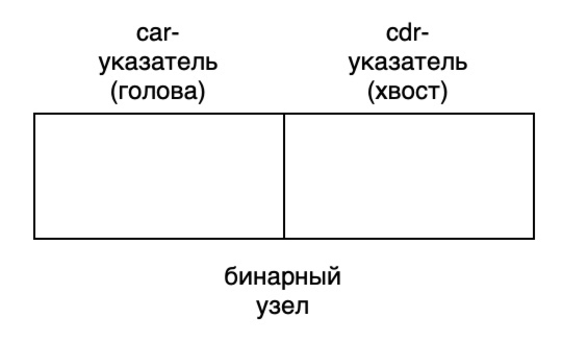
\includegraphics[width=0.3\linewidth]{./images/b.pdf}
    \captionof{figure}{Списковая ячейка}
    \label{img:3}
  \end{tabular}
\end{table}


\section{Трактовка элементов списка}
При обработке списков первый элемент воспринимается интерпретатором как название функции, все остальные~---~ее аргументы (список трактуется как вычислимая форма). Количество элементов, не считая первого~---~названия функции, должно совпадать с количеством входных аргументов указанной функции.

В случае если перед скобкой применяется блокировка вычислений (\texttt{`} или \texttt{quota}), результатом является все, что стоит после блокировки.

\begin{code}
\begin{minted}{lisp}
> (cons 1 2)
(1 . 2)
\end{minted}
\end{code}

\begin{code}
\begin{minted}{lisp}
> (cons 1 2 3)
EVAL: too many arguments given to CONS: (CONS 1 2 3)
\end{minted}
\end{code}

\begin{code}
\begin{minted}{lisp}
> `(cons 1 2)
(CONS 1 2)
\end{minted}
\end{code}


\section{Порядок реализации программы}
\begin{enumerate}
	\item Ожидает ввода S-выражения.
	\item Передает введенное S-выражение функции \texttt{eval}.
	\item Выводит полученный результат.
\end{enumerate}

\begin{table}[h!]
  \centering
  \begin{tabular}{p{1\linewidth}}
    \centering
    \includegraphics[width=0.6\linewidth]{./images/eval.pdf}
    \captionof{figure}{Диаграмма работы \texttt{eval}}
    \label{img:3}
  \end{tabular}
\end{table}

\newpage


\section{Способы определения функции}
Функцию можно определить двумя способами: неименованную с помощью \texttt{lambda} и именованную с помощью \texttt{defun}.

\begin{code}
\begin{minted}{lisp}
(lambda (x_1 x_2 ... x_n) f)
\end{minted}
\end{code}

\begin{itemize}
	\item \texttt{f}~---~тело функции;
	\item \texttt{x\_i}~---~формальные параметры.
\end{itemize}

\begin{code}
\begin{minted}{lisp}
(defun <имя> [lambda] (x_1 x_2 ... x_n) f)
\end{minted}
\end{code}

\begin{itemize}
	\item \texttt{f}~---~тело функции;
	\item \texttt{x\_i}~---~формальные параметры. 
\end{itemize}

Тогда имя будет ссылкой на описание функции.


\section{Работа со списками}
Ниже перечислены наиболее часто используемые для работы со списками функции.

\subsection{Создание}
Список можно создать несколькими способами. 

\begin{enumerate}

\item Базисная функция \texttt{cons} может создавать список, если её второй аргумент является списком.
 
\begin{code}
\begin{minted}{lisp}
> (cons 1 `(2 3 4))
(1 2 3 4)
\end{minted}
\end{code}

\item Функция \texttt{list} также создаёт список, принимая на вход неопределённое количество аргументов.

\begin{code}
\begin{minted}{lisp}
> (list 1 `(2 3 4) 5 6)
(1 (2 3 4) 5 6)
\end{minted}
\end{code}

\item Функция \texttt{last} возвращает список, содержащий последний элемент в списке.

\begin{code}
\begin{minted}{lisp}
> (last `(1 2 3))
(3)
\end{minted}
\end{code}

\item \texttt{append} принимает произвольное количество аргументов-списков и соединяет элементы верхнего уровня всех списков в один список. В результате должен быть построен новый список.

\begin{code}
\begin{minted}{lisp}
> (append (list 1 2) (list 3 4))
(1 2 3 4)
\end{minted}
\end{code}

\end{enumerate}

\subsection{Изменение}

\begin{enumerate} 
\item Конкатенация~---~\texttt{nconc}. Похожа на \texttt{append}, но в отличие от неё <<ломает>> свои аргументы, не создавая копии списковых ячеек.

\begin{code}
\begin{minted}{lisp}
> (setf x (list 1 2))
(1 2)
> (nconc x (list 3 4))
(1 2 3 4)
> x
(1 2 3 4)
\end{minted}
\end{code}

\item \texttt{reverse}~---~выполняет разворот списка по верхнему уровню списковых ячеек. Создает копию, не <<ломая>> аргумент. 

\begin{code}
\begin{minted}{lisp}
> (setf x (list 1 2))
(1 2)
> (reverse x)
(4 3 2 1)
> x
(1 2 3 4)
\end{minted}
\end{code}

\item \texttt{nreverse}~---~работает аналогично, но без создания копий.

\begin{code}
\begin{minted}{lisp}
> (setf x (list 1 2))
(1 2)
> (nreverse x)
(4 3 2 1)
> x
(4 3 2 1)
\end{minted}
\end{code}
\end{enumerate}

\subsection{Селекторы}
Функция \texttt{car} используется для получения \texttt{car}-указателя~---~указателя на голову списка. Функция \texttt{cdr} используется для получения \texttt{cdr}-указателя~---~указателя на хвост списка.

\begin{code}
\begin{minted}{lisp}
(car `(1 2 3 4))
1
\end{minted}
\end{code}

\begin{code}
\begin{minted}{lisp}
> (cdr `(1 2 3 4))
(2 3 4)
\end{minted}
\end{code}

Также, можно использовать композицию функций.

\begin{code}
\begin{minted}{lisp}
> (caddr `(1 2 3 4))
3
\end{minted}
\end{code}

\begin{code}
\begin{minted}{lisp}
> (caadr `(1 (2 5) 3 4))
2
\end{minted}
\end{code}


\newpage

\chapter{Практическая часть}
\section{Задание 1}
\subsection*{Задание}
Чем принципиально отличаются функции cons, list, append? Пусть 

\begin{code}
\begin{minted}{lisp}
(setf lst1 `( a b c))
(setf lst2 `( d e))
\end{minted}
\end{code}

Каковы результаты вычисления следующих выражений?

\begin{enumerate}
	\item \texttt{(cons lst1 lst2)}
	\item \texttt{(list lst1 lst2)}
	\item \texttt{(append lst1 lst2)}
\end{enumerate}

\subsection*{Решение}
\begin{enumerate}
	\item \texttt{((A B C) D E)}
	\item \texttt{((A B C) (D E))}
	\item \texttt{(A B C D E)}
\end{enumerate}


\section{Задание 2}
\subsection*{Задание}
Каковы результаты вычисления следующих выражений, и почему?

\begin{enumerate}
	\item \texttt{(reverse `(a b c))}
	\item \texttt{(reverse `(a b (c (d))))}
	\item \texttt{(reverse `(a))}
	\item \texttt{(last `(a b c))}
	\item \texttt{(last `(a))}
	\item \texttt{(last `((a b c)))}
	\item \texttt{(reverse ())}
	\item \texttt{(reverse `((a b c)))}
	\item \texttt{(last `(a b (c)))}
	\item \texttt{(last ())}
\end{enumerate}

\subsection*{Решение}
\begin{enumerate}
	\item \texttt{(C B A)}
	\item \texttt{((C (D)) B A)}
	\item \texttt{(A)}
	\item \texttt{(C)}
	\item \texttt{(A)}
	\item \texttt{((A B C))}
	\item \texttt{NIL}
	\item \texttt{((A B C))}
	\item \texttt{((C))}
	\item \texttt{NIL}
\end{enumerate}


\section{Задание 3}
\subsection*{Задание}
Написать, по крайней мере, два варианта функции, которая возвращает последний элемент своего списка-аргумента.

\subsection*{Решение}
\begin{code}
\begin{minted}{lisp}
(defun f1 (x) (car (last x)))
\end{minted}
\end{code}

\begin{code}
\begin{minted}{lisp}
(defun f2 (x) (car (reverse x)))
\end{minted}
\end{code}


\section{Задание 4}
\subsection*{Задание}
Написать, по крайней мере, два варианта функции, которая возвращает свой список аргумент без последнего элемента.

\subsection*{Решение}
\begin{code}
\begin{minted}{lisp}
(defun f3 (x) (reverse (cdr (reverse x))))
\end{minted}
\end{code}

\begin{code}
\begin{minted}{lisp}
(defun f4 (x) 
	(if (<= (length x) 1)
		nil
		(cons (car x) (f4 (cdr x)))	
	)
)
\end{minted}
\end{code}


\section{Задание 5}
\subsection*{Задание}
Напишите функцию \texttt{swap-first-last}, которая переставляет в списке-аргументе первый и последний элементы.

\subsection*{Решение}
\begin{code}
\begin{minted}{lisp}
(defun f5 (x)
	(append (last x) (cdr (f4 x)) (list (first x)))
)
\end{minted}
\end{code}


\section{Задание 6}
\subsection*{Задание}
Написать простой вариант игры в кости, в котором бросаются две правильные кости. Если сумма выпавших очков равна 7 или 11~---~выигрыш, если выпало (1,1) или (6,6) — игрок имеет право снова бросить кости, во всех остальных случаях ход переходит ко второму игроку, но запоминается сумма выпавших очков. Если второй игрок не выигрывает абсолютно, то выигрывает тот игрок, у которого больше очков. Результат игры и значения выпавших костей выводить на экран с помощью функции \texttt{print}.

\subsection*{Решение}
\begin{code}
\begin{minted}{lisp}
(defun dice ()
	(+ (random 6) 1)
)

(defun is_retry (p)
	(or (equal p (cons 6 6)) (equal p (cons 1 1)))
)
\end{minted}
\end{code}

\newpage

\begin{code}
\begin{minted}{lisp}
(defun player_dice (n) 
	(let ((pair (cons (dice) (dice)))) 
		(print (list n `played pair))
		(cond
			((is_retry pair) (player_dice n))
			(t (+ (car pair) (cdr pair)))
		)
	)
)

(defun is_win (s)
	(or (= s 7) (= s 11))
)

(defun play ()
	(let ((s1 (player_dice 1)) (s2 (player_dice 2)))
		(cond
			((is_win s1) (print "1 absolute win"))
			((is_win s2) (print "2 absolute win"))
			((> s1 s2) (print "1 win"))
			((< s1 s2) (print "2 win"))
			(t (print "nobody win"))
		)
		nil
	)
)
\end{minted}
\end{code}


\section{Задание 7}
\subsection*{Задание}
Написать функцию, которая по своему списку-аргументу \texttt{lst} определяет является ли он палиндромом (то есть равны ли \texttt{lst} и \texttt{(reverse lst)}).

\subsection*{Решение}
\begin{code}
\begin{minted}{lisp}
(defun f6 (x) (equalp x (reverse x)))
\end{minted}
\end{code}


\section{Задание 8}
\subsection*{Задание}
Напишите свои необходимые функции, которые обрабатывают таблицу из 4-х точечных пар:
(страна . столица), и возвращают по стране~---~столицу, а по столице~---~страну.

\subsection*{Решение}
\begin{code}
\begin{minted}{lisp}
(defun capital (table c)
        (cdr (assoc c table :test #'equalp))
)
\end{minted}
\end{code}

\begin{code}
\begin{minted}{lisp}
(defun country (table c)
        (car (rassoc c table :test #'equalp))
)
\end{minted}
\end{code}

\section{Задание 9}
\subsection*{Задание}
Напишите функцию, которая умножает на заданное число-аргумент первый числовой элемент списка из заданного 3-х элементного списка-аргумента, когда

\begin{enumerate}
	\item все элементы списка~---~числа;
	\item элементы списка~---~любые объекты.
\end{enumerate}

\subsection*{Решение}
\begin{code}
\begin{minted}{lisp}
(defun f7 (l n)
	(cond
		((not (listp l)) nil)
		((not (numberp n)) nil)
		((not (= (length l) 3)) nil)
		(t (list (* (first l) n) (second l) (third l)))
	)
)
\end{minted}
\end{code}

\begin{code}
\begin{minted}{lisp}
(defun f8 (l n)
	(cond
		((not (listp l)) nil)
		((not (numberp n)) nil)
		((not (= (length l) 3)) nil)
		((numberp (first l)) (list (* (first l) n) (second l) 
		(third l)))
		((numberp (second l)) (list (first l) (* (second l) n) 
		(third l)))
		((numberp (third l)) (list (first l) (second l) 
		(* (third l) n)))
		(t nil)
	)
)
\end{minted}
\end{code}

\newpage